\chapter{Biomolekul: Asam Amino, Gula, Lipid, dan Nukleotida}\label{ch:b2:biomolecules}

Sebuah pemanis yang lazim, jauh lebih manis daripada gula, terdiri atas dua
asam amino yang disambungkan oleh satu ikatan amida, salah satunya dalam
bentuk metil esternya: asam aspartat dan fenilalanina, keduanya dengan
konfigurasi yang dipakai sel-sel hidup. Molekul-molekul kehidupan dibangun
dari beberapa keluarga satuan kecil, yaitu asam amino, gula, \omterm{def:b2:biomolecules:lipid}{asam lemak}, dan
\omterm{def:b2:biomolecules:nucleotide}{nukleotida}, yang disambungkan oleh reaksi-reaksi dari bab-bab sebelumnya:
amida, asetal, ester. Bab ini membacanya seperti seorang kimiawan organik:
gugus fungsi, stereokimia, perilaku asam--basa, dan reaksi-reaksi yang
menyambung dan memotongnya.
% ledger: use:aspartame

\begin{recall}
Jilid Tahun 1: aturan CIP, proyeksi Fischer, kekiralan, hemiasetal dan
asetal, $\mathrm pK_a$
dan diagram distribusi, molekul amfifilik, hukum Biot. \Cref{ch:b2:acyl-substitution}:
amida, ester, \omterm{def:b2:acyl-substitution:saponification}{saponifikasi}, asam teraktivasi. \Cref{ch:b2:amines}: amina
sebagai basa. \Cref{ch:b2:retrosynthesis}: gugus pelindung dalam sebuah
jalur.
\end{recall}

\section{Asam amino}

\begin{definition}[Asam amino]\label{def:b2:biomolecules:amino-acid}
Sebuah \emph{asam $\alpha$-amino}\index{asam alfa-amino@asam $\alpha$-amino}
\ce{H2N-CHR-COOH} membawa gugus amino dan gugus asam karboksilat pada karbon
yang sama; \ce{R} adalah \emph{rantai
samping}\index{rantai samping}-nya. Dalam air di sekitar pH netral, asam
amino berada sebagai \emph{zwitterion}\index{zwitterion},
\ce{H3N+-CHR-COO-}, yang membawa satu muatan positif dan satu muatan
negatif. Yang disebut \emph{titik
isoelektrik}\index{titik isoelektrik} pI adalah pH tempat muatan bersih
rata-ratanya nol.
\end{definition}

Dua puluh asam amino membangun protein makhluk hidup. Semuanya kecuali
glisina (\ce{R = H}) bersifat kiral, dan yang alami mempunyai konfigurasi L
(\cref{def:b2:biomolecules:d-l}). \omterm{def:b2:biomolecules:amino-acid}{Rantai sampingnya} memilah asam-asam amino
itu menjadi beberapa keluarga: nonpolar (alanina, \ce{R = CH3}; fenilalanina,
\ce{R = CH2C6H5}), polar, asam (asam aspartat dan glutamat, dengan gugus
karboksilat kedua) dan basa (lisina, dengan gugus amino kedua; histidina,
dengan cincin imidazol).

\begin{proposition}[Titik isoelektrik]\label{prop:b2:biomolecules:pi}
Untuk asam amino dengan \omterm{def:b2:biomolecules:amino-acid}{rantai samping} yang tidak asam dan tidak basa,
$\mathrm{pI} = (\mathrm pK_{a1} +
\mathrm pK_{a2})/2$, dengan $\mathrm pK_{a1}$ milik gugus karboksilat dan
$\mathrm pK_{a2}$ milik gugus amonium. Untuk \omterm{def:b2:biomolecules:amino-acid}{rantai samping} yang asam atau
basa, pI adalah rata-rata kedua $\mathrm pK_a$ yang mengapit bentuk netral.
\end{proposition}

\begin{proof}
Tuliskan \ce{H2A+} untuk kation, \ce{HA} untuk \omterm{def:b2:biomolecules:amino-acid}{zwitterion}, dan \ce{A-} untuk
anion. Muatan bersihnya nol jika $[\ce{H2A+}] = [\ce{A-}]$. Dari $K_{a1} = [\ce{HA}]h/[\ce{H2A+}]$ dan $K_{a2} =
[\ce{A-}]h/[\ce{HA}]$, dengan $h = [\ce{H3O+}]$, rasio $[\ce{H2A+}]/[\ce{A-}] = h^2/(K_{a1}K_{a2})$
sama dengan 1 untuk $h^2 = K_{a1}K_{a2}$, yaitu $\mathrm{pH} = (\mathrm pK_{a1} + \mathrm pK_{a2})/2$.
Dengan gugus terionkan ketiga, argumen yang sama berlaku untuk kedua
kesetimbangan di kedua sisi bentuk netral, karena gugus ketiga itu lalu
berada seluruhnya dalam satu keadaan.
\end{proof}

Untuk glisina, $\mathrm pK_{a1} = 2.35$ dan $\mathrm pK_{a2} = 9.78$: pI $\approx 6.1$.
Asam aspartat (2.0, 3.9, 9.9) mempunyai pI $\approx 3.0$; lisina (2.2, 9.1, 10.7) mempunyai pI $\approx 9.9$.
% ledger: pka:glycine1, pka:glycine2, pka:asp1, pka:asp2, pka:asp3, pka:lys1, pka:lys2, pka:lys3

\begin{omfigure}
\begin{tikzpicture}
\begin{axis}[width=0.47\linewidth, height=5cm, xmin=0, xmax=14, ymin=-2.2, ymax=2.2,
  xlabel={pH}, ylabel={muatan bersih}, label style={font=\small}, tick label style={font=\scriptsize},
  xtick={0,2,4,6,8,10,12,14}, ytick={-2,-1,0,1,2}, grid=major, grid style={black!12},
  legend style={font=\scriptsize, at={(0.5,1.03)}, anchor=south}, legend columns=3]
\addplot[omDef, thick] table[x=pH, y=gly] {figdata/out/bachelor-2-amino-acid-charge-a.dat};
\addplot[omThm, thick] table[x=pH, y=asp] {figdata/out/bachelor-2-amino-acid-charge-a.dat};
\addplot[omMeth, thick] table[x=pH, y=lys] {figdata/out/bachelor-2-amino-acid-charge-a.dat};
\legend{glisina, asam aspartat, lisina}
\end{axis}
\end{tikzpicture}\hfill
\begin{tikzpicture}
\begin{axis}[width=0.47\linewidth, height=5cm, xmin=0, xmax=14, ymin=0, ymax=1.05,
  xlabel={pH}, ylabel={fraksi}, label style={font=\small}, tick label style={font=\scriptsize},
  xtick={0,2,4,6,8,10,12,14},
  legend style={font=\scriptsize, at={(0.5,1.03)}, anchor=south}, legend columns=3]
\addplot[omThm, thick] table[x=pH, y=cation] {figdata/out/bachelor-2-amino-acid-charge-b.dat};
\addplot[omDef, thick] table[x=pH, y=zwitterion] {figdata/out/bachelor-2-amino-acid-charge-b.dat};
\addplot[omMeth, thick] table[x=pH, y=anion] {figdata/out/bachelor-2-amino-acid-charge-b.dat};
\legend{kation, zwitterion, anion}
\end{axis}
\end{tikzpicture}

{\small Kiri: muatan bersih tiga asam amino terhadap pH, dari $\mathrm pK_a$-nya
pada \qty{25}{\degreeCelsius}; setiap kurva memotong nol pada pI. Kanan:
ketiga bentuk glisina,
\ce{H3N+CH2COOH}, \ce{H3N+CH2COO-}, dan \ce{H2NCH2COO-}; \omterm{def:b2:biomolecules:amino-acid}{zwitterion} dominan
dari sekitar pH 3 sampai pH 9.}
% figdata: bachelor-2/amino-acid-charge.py parts a, b
\end{omfigure}

\begin{method}[Muatan bersih pada pH tertentu]\label{met:b2:biomolecules:charge}
\begin{enumerate}
  \item Daftarlah setiap gugus terionkan beserta $\mathrm pK_a$-nya: \ce{NH3+} dan \ce{COOH}
        ujung, serta rantai-rantai samping yang terionkan.
  \item Untuk setiap gugus, bandingkan pH dan $\mathrm pK_a$: sebuah gugus
        sebagian besar terprotonasi di bawah $\mathrm pK_a$-nya, sebagian
        besar terdeprotonasi di atasnya (dengan selisih lebih dari 1 satuan:
        lebih dari 90~\%).
  \item Jumlahkan muatannya: \ce{NH3+} $+1$, \ce{NH2} 0, \ce{COOH} 0, \ce{COO-} $-1$ (imidazolium $+1$).
  \item Di dekat sebuah $\mathrm pK_a$, hitunglah gugus itu bermuatan
        separuh; untuk nilai yang eksak, pakailah fraksi
        $1/(1 + 10^{\mathrm pK_a - \mathrm{pH}})$.
\end{enumerate}
\end{method}

\section{Peptida}

\begin{definition}[Peptida]\label{def:b2:biomolecules:peptide}
Ikatan amida yang terbentuk antara gugus karboksilat sebuah asam amino dan
gugus amino asam amino lain disebut \emph{ikatan peptida}\index{ikatan peptida};
rantai asam amino yang disambungkan oleh ikatan-ikatan peptida disebut
\emph{peptida}\index{peptida} (protein jika panjang), yang ditulis dari ujung
amino bebasnya (ujung-N) sampai ujung karboksilat bebasnya (ujung-C). Yang
disebut \emph{kopling peptida}\index{kopling peptida} membentuk ikatan
peptida di laboratorium dengan sebuah \emph{pereaksi kopling}\index{pereaksi kopling},
yaitu pereaksi yang mengubah gugus karboksilat menjadi turunan teraktivasi
dalam kondisi lunak (misalnya sebuah karbodiimida).
\end{definition}

\begin{omfigure}
\setchemfig{atom sep=1.9em}
\schemestart
\chemfig{R-C(=[2]O)-N(-[6]H)-R'}
\arrow{<->}
\chemfig{R-C(-[2]\chemabove{O}{\scriptstyle -})=\chemabove{N}{\scriptstyle +}(-[6]H)-R'}
\schemestop
\par\vspace{6pt}

{\small Kedua struktur resonansi \omterm{def:b2:biomolecules:peptide}{ikatan peptida}. Pasangan elektron bebas
nitrogen dipakai bersama dengan karbonil: ikatan \ce{C-N} mempunyai sifat
ikatan rangkap parsial, dan keenam atom C, C, O, N, H, C terletak pada satu
bidang.}
\end{omfigure}

\begin{proposition}[Ikatan yang planar]\label{prop:b2:biomolecules:planar}
\omterm{def:b2:biomolecules:peptide}{Ikatan peptida} bersifat planar, rotasi pada ikatan \ce{C-N} terhambat, dan
nitrogen amida tidak bersifat basa dan tidak nukleofilik.
\end{proposition}

\begin{proof}[Argumen]
Struktur resonansi kedua memberi ikatan \ce{C-N} sebagian sifat ikatan
rangkap: memutarnya akan memutus tumpang-tindih pasangan elektron bebas
nitrogen dengan sistem $\pi$ \ce{C=O}, yang memerlukan energi, sehingga
atom-atom di sekitarnya tetap berada pada satu bidang, dengan susunan trans
(kedua karbon rantai pada sisi ikatan \ce{C-N} yang berseberangan) sebagai
susunan yang lazim. Pasangan elektron bebas yang terlibat dalam resonansi
tidak tersedia bagi proton atau elektrofil, seperti pada setiap amida
(\cref{ch:b2:acyl-substitution}). Protein melipat di sekitar rantai-rantai
bidang kaku ini.
\end{proof}

\begin{proposition}[Mengapa melindungi dan mengaktifkan]\label{prop:b2:biomolecules:coupling}
Membuat satu dipeptida tertentu dari dua asam amino memerlukan perlindungan
gugus-gugus yang tidak boleh bereaksi sekaligus aktivasi gugus karboksilat
yang harus bereaksi.
\end{proposition}

\begin{proof}[Argumen]
Asam karboksilat dan amina yang dicampur pada suhu kamar menghasilkan garam,
bukan amida; pemanasan untuk mengusir air juga akan merasemisasi asam-asam
amino itu. Karena itu diperlukan aktivasi (\omterm{def:b2:acyl-substitution:derivative}{asil klorida}, anhidrida, atau
\omterm{def:b2:biomolecules:peptide}{pereaksi kopling}). Tetapi setiap asam amino mempunyai kedua gugus itu:
mengaktifkan campuran glisina dan alanina akan menghasilkan Gly--Ala,
Ala--Gly, Gly--Gly, Ala--Ala, dan rantai-rantai yang lebih panjang.
Memblokir amina asam amino pertama dan asam asam amino kedua hanya
menyisakan satu ikatan yang mungkin.
\end{proof}

\begin{method}[Sintesis sebuah dipeptida]\label{met:b2:biomolecules:peptide}
\begin{enumerate}
  \item Lindungi gugus amino asam amino ujung-N (sebagai karbamat, misalnya
        gugus \textit{tert}-butoksikarbonil).
  \item Lindungi gugus karboksilat asam amino ujung-C (sebagai metil atau
        benzil ester), dan setiap \omterm{def:b2:biomolecules:amino-acid}{rantai samping} yang reaktif.
  \item Aktifkan gugus karboksilat yang bebas dengan \omterm{def:b2:biomolecules:peptide}{pereaksi kopling} dan
        tambahkan pasangan yang terlindungi: satu \omterm{def:b2:biomolecules:peptide}{ikatan peptida} terbentuk.
  \item Lepaskan gugus-gugus pelindungnya, sebaiknya sehimpunan gugus
        ortogonal (\cref{def:b2:retrosynthesis:orthogonal}); untuk
        melanjutkan, lepaskan hanya pelindung amina dan ulangi.
\end{enumerate}
\end{method}

Mengulangi siklus itu berkali-kali dalam larutan akan memerlukan pemurnian
pada setiap tahap. Dalam sintesis fase padat, rantai yang sedang tumbuh
ditambatkan melalui ujung-C-nya pada sebutir manik \omterm{def:b2:polymer-synthesis:polymer}{polimer}; pereaksi
berlebih dan produk samping dicuci setelah setiap kopling, dan \omterm{def:b2:biomolecules:peptide}{peptida} yang
sudah jadi dipotong dari penyangganya di akhir.

\begin{omfigure}
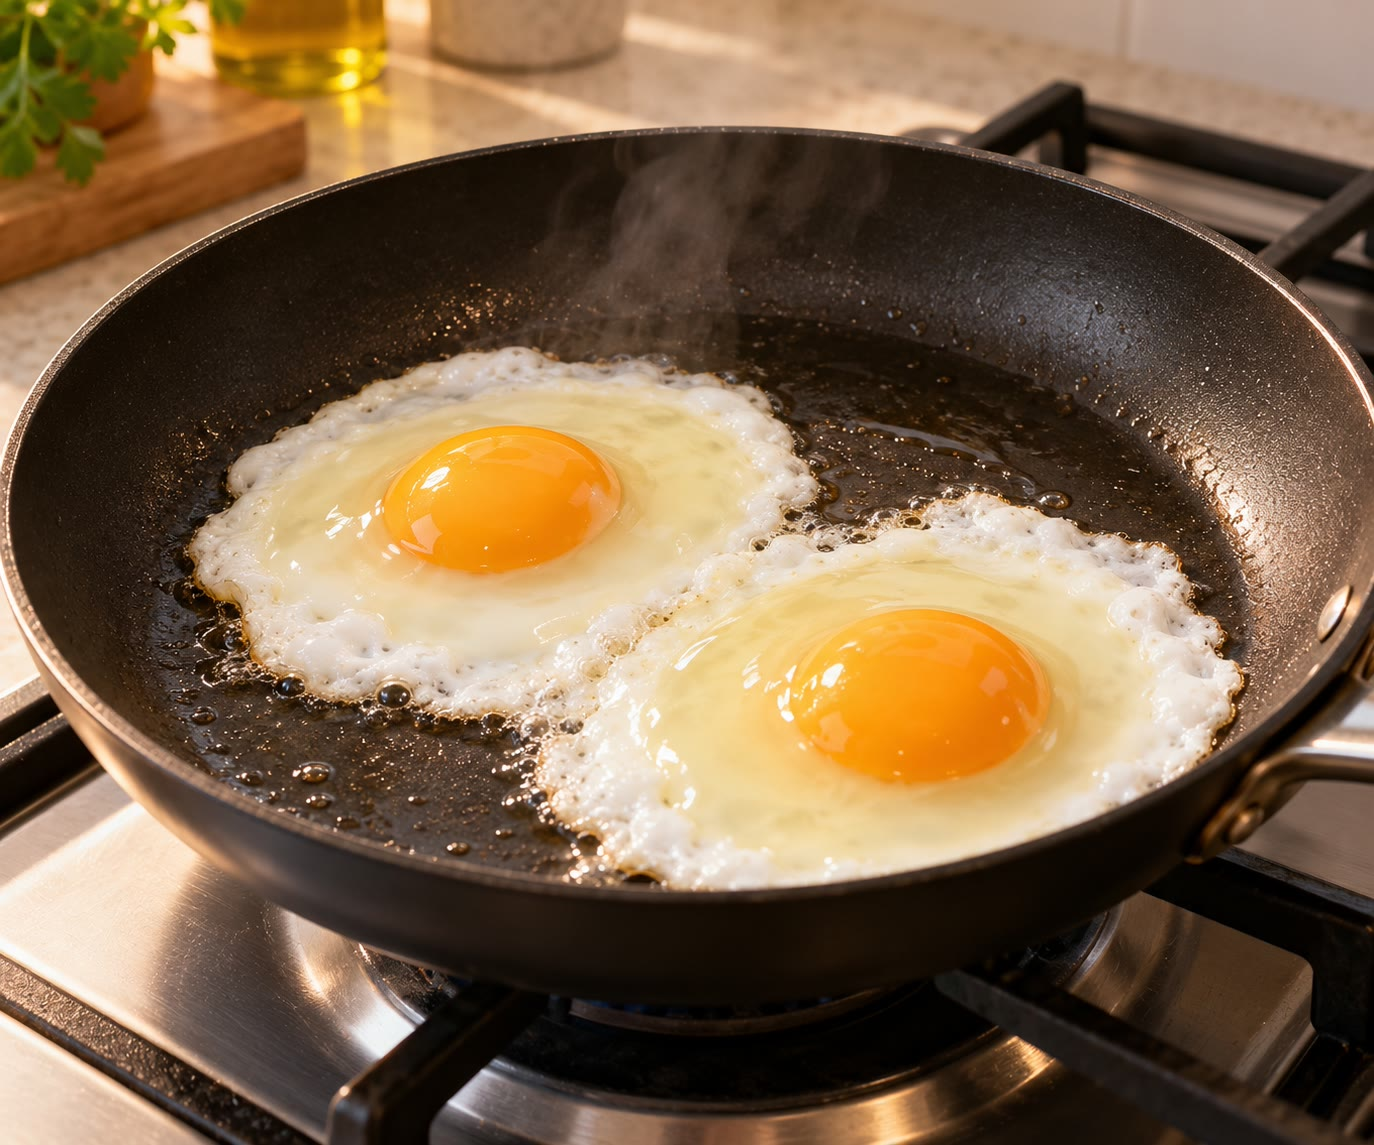
\includegraphics[width=0.5\linewidth]{images/book3/ai/b2-30-eggs.jpg}

{\small Telur yang sedang digoreng. Protein-protein putih telur membuka
lipatannya pada pemanasan dan saling berikatan: cairan yang tembus cahaya
berubah menjadi padatan putih yang opak. Tidak ada \omterm{def:b2:biomolecules:peptide}{ikatan peptida} yang
putus; perubahannya terletak pada cara rantai-rantai itu terlipat
(ilustrasi).}
\end{omfigure}

\section{Karbohidrat}

\begin{definition}[D dan L]\label{def:b2:biomolecules:d-l}
Gula atau asam amino digambar dalam proyeksi Fischer dengan karbonnya yang
paling teroksidasi di atas. Senyawa itu D jika \ce{OH} pada pusat
stereogenik yang paling jauh dari atas (atau, untuk asam $\alpha$-amino,
\ce{NH2} pada karbon $\alpha$) mengarah ke kanan, dan L jika mengarah ke
kiri. Deskriptor ini membandingkan konfigurasi dengan konfigurasi
gliseraldehida; deskriptor ini bukan deskriptor CIP.
\end{definition}

\begin{definition}[Monosakarida]\label{def:b2:biomolecules:sugar}
Yang disebut \emph{monosakarida}\index{monosakarida} adalah aldehida atau
keton polihidroksi, biasanya
\ce{C_nH_{2n}O_n} dengan $n$ dari 3 sampai 7, yang tidak dapat dihidrolisis
menjadi gula yang lebih kecil. Sebuah \emph{aldosa}\index{aldosa} mempunyai
gugus aldehida pada C1, sebuah \emph{ketosa}\index{ketosa} mempunyai gugus
keton, biasanya pada C2. Glukosa adalah aldoheksosa, fruktosa ketoheksosa.
\end{definition}

Dalam air, aldoheksosa hampir seluruhnya berbentuk siklik: \ce{OH} pada C5
beradisi pada aldehida dan membentuk cincin hemiasetal beranggota enam
(piranosa). Siklisasi itu menciptakan pusat stereogenik baru pada C1.

\begin{definition}[Anomer]\label{def:b2:biomolecules:anomer}
Dalam \emph{proyeksi Haworth}\index{proyeksi Haworth}, cincin gula siklik
digambar datar, tegak lurus halaman, dengan oksigennya di belakang kanan dan
substituen-substituennya di atas atau di bawah cincin. Karbon hemiasetal
(C1 sebuah \omterm{def:b2:biomolecules:sugar}{aldosa}) disebut \emph{karbon anomerik}\index{karbon anomerik};
kedua konfigurasi yang dapat diambilnya menghasilkan dua diastereoisomer,
yaitu \emph{anomer}\index{anomer}: untuk gula D,
$\alpha$ mempunyai \ce{OH} anomerik di bawah cincin (berseberangan dengan
\ce{CH2OH}), $\beta$ di atas. Dalam air, anomer-anomer saling berubah
melalui rantai terbuka, dan rotasi optik anomer yang baru dilarutkan
bergeser menuju nilai kesetimbangan: \emph{mutarotasi}\index{mutarotasi}.
\end{definition}

\begin{omfigure}
\setchemfig{atom sep=1.7em}
\begin{minipage}[c]{0.24\linewidth}\centering
\chemfig{CHO-[6]C(-[4]H)(-[0]OH)-[6]C(-[4,,,2]HO)(-[0]H)-[6]C(-[4]H)(-[0]OH)-[6]C(-[4]H)(-[0]OH)-[6]CH_2OH}
\end{minipage}%
\begin{minipage}[c]{0.37\linewidth}\centering
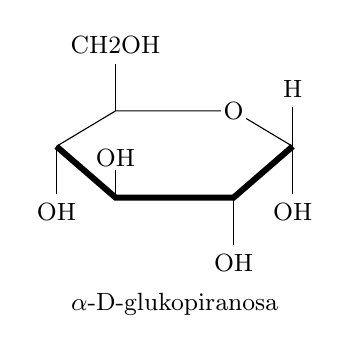
\begin{tikzpicture}[x=1cm, y=1cm, font=\small]
\coordinate (C4) at (-1.5,0); \coordinate (C3) at (-0.75,-0.65); \coordinate (C2) at (0.75,-0.65);
\coordinate (C1) at (1.5,0); \coordinate (O) at (0.75,0.45); \coordinate (C5) at (-0.75,0.45);
\draw (C5) -- (O) -- (C1); \draw (C4) -- (C5);
\draw[line width=2.2pt] (C4) -- (C3) -- (C2) -- (C1);
\node[fill=white, inner sep=1pt] at (O) {O};
\draw (C5) -- ++(0,0.6) node[above] {\ce{CH2OH}};
\draw (C1) -- ++(0,-0.6) node[below] {OH}; \draw (C1) -- ++(0,0.5) node[above] {H};
\draw (C2) -- ++(0,-0.6) node[below] {OH}; \draw (C3) -- ++(0,0.35) node[above, inner sep=1pt] {OH};
\draw (C4) -- ++(0,-0.6) node[below] {OH};
\node at (0,-2.0) {$\alpha$-D-glukopiranosa};
\end{tikzpicture}
\end{minipage}%
\begin{minipage}[c]{0.37\linewidth}\centering
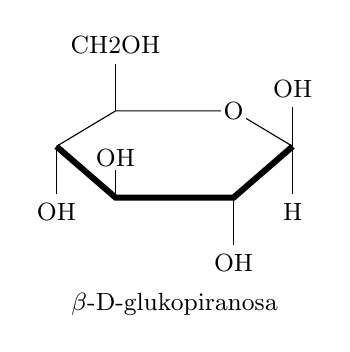
\begin{tikzpicture}[x=1cm, y=1cm, font=\small]
\coordinate (C4) at (-1.5,0); \coordinate (C3) at (-0.75,-0.65); \coordinate (C2) at (0.75,-0.65);
\coordinate (C1) at (1.5,0); \coordinate (O) at (0.75,0.45); \coordinate (C5) at (-0.75,0.45);
\draw (C5) -- (O) -- (C1); \draw (C4) -- (C5);
\draw[line width=2.2pt] (C4) -- (C3) -- (C2) -- (C1);
\node[fill=white, inner sep=1pt] at (O) {O};
\draw (C5) -- ++(0,0.6) node[above] {\ce{CH2OH}};
\draw (C1) -- ++(0,0.5) node[above] {OH}; \draw (C1) -- ++(0,-0.6) node[below] {H};
\draw (C2) -- ++(0,-0.6) node[below] {OH}; \draw (C3) -- ++(0,0.35) node[above, inner sep=1pt] {OH};
\draw (C4) -- ++(0,-0.6) node[below] {OH};
\node at (0,-2.0) {$\beta$-D-glukopiranosa};
\end{tikzpicture}
\end{minipage}
\par\vspace{6pt}

{\small D-Glukosa. Kiri: rantai terbuka dalam proyeksi Fischer, \ce{OH} pada
C5 di kanan (D). Tengah dan kanan: kedua \omterm{def:b2:biomolecules:anomer}{anomer} piranosa dalam \omterm{def:b2:biomolecules:anomer}{proyeksi
Haworth}; gugus-gugus di sebelah kanan proyeksi Fischer mengarah ke bawah,
gugus-gugus di sebelah kiri mengarah ke atas, dan C5 membawa \ce{CH2OH} ke
atas. Kedua \omterm{def:b2:biomolecules:anomer}{anomer} hanya berbeda pada C1. Hidrogen-hidrogen pada C2 sampai
C5 tidak digambar.}
\end{omfigure}

\begin{method}[Dari Fischer ke Haworth (D-aldopiranosa)]\label{met:b2:biomolecules:haworth}
\begin{enumerate}
  \item Gambarlah cincin dengan O di belakang kanan, C1 di kanan, lalu C2,
        C3, C4 searah jarum jam di sepanjang bagian depan dan kiri, C5 di
        belakang kiri.
  \item Gugus-gugus di sebelah kanan dalam proyeksi Fischer mengarah ke
        bawah, gugus-gugus di sebelah kiri mengarah ke atas.
  \item Pada C5 (deret D), \ce{CH2OH} mengarah ke atas.
  \item Pada C1, \ce{OH} mengarah ke bawah untuk $\alpha$, ke atas untuk $\beta$.
\end{enumerate}
\end{method}

\begin{proposition}[Kesetimbangan mutarotasi]\label{prop:b2:biomolecules:mutarotation}
Jika rotasi spesifik \omterm{def:b2:biomolecules:anomer}{anomer-anomer} murni adalah $[\alpha]_\alpha$ dan
$[\alpha]_\beta$ dan rotasi spesifik campuran kesetimbangan adalah
$[\alpha]_{\mathrm{eq}}$, fraksi mol \omterm{def:b2:biomolecules:anomer}{anomer} $\alpha$ pada kesetimbangan
adalah
\begin{equation*}
x_\alpha = \frac{[\alpha]_{\mathrm{eq}} - [\alpha]_\beta}{[\alpha]_\alpha - [\alpha]_\beta}.
\end{equation*}
\end{proposition}

\begin{proof}
Rantai terbuka hanya merupakan fraksi yang sangat kecil dari campuran dan
diabaikan. Rotasi kedua \omterm{def:b2:biomolecules:anomer}{anomer} saling menjumlah sebanding dengan
konsentrasinya (hukum Biot, jilid Tahun 1); karena keduanya mempunyai massa
molar yang sama, $[\alpha]_{\mathrm{eq}} = x_\alpha[\alpha]_\alpha + (1 - x_\alpha)[\alpha]_\beta$,
yang diselesaikan untuk $x_\alpha$.
\end{proof}

D-Glukosa dalam kesetimbangan di dalam air mempunyai $[\alpha] = +52.7$ (dalam \unit{\degree\,dm^{-1}\,g^{-1}\,mL}).
Dengan rotasi \omterm{def:b2:biomolecules:anomer}{anomer} $+112$ dan $+18.7$ (data latihan), $x_\alpha = (52.7 - 18.7)/(112 - 18.7)
\approx 0.36$: sekitar 36~\% $\alpha$ dan 64~\% $\beta$. \omterm{def:b2:biomolecules:anomer}{Anomer} $\beta$,
dengan semua substituennya ekuatorial pada konformasi kursi, adalah yang
lebih stabil.
% ledger: rot:glucose-eq

\begin{definition}[Glikosida]\label{def:b2:biomolecules:glycoside}
Yang disebut \emph{glikosida}\index{glikosida} adalah asetal yang terbentuk
ketika \ce{OH} anomerik sebuah gula digantikan oleh gugus \ce{OR} dari
sebuah alkohol, sering gula lain; ikatan dari \omterm{def:b2:biomolecules:anomer}{karbon anomerik} ke oksigen itu
adalah \emph{ikatan glikosidik}\index{ikatan glikosidik}. Yang disebut
\emph{gula pereduksi}\index{gula pereduksi}
adalah gula yang mereduksi pengoksidasi lunak seperti larutan Fehling atau
pereaksi Tollens.
\end{definition}

\begin{proposition}[Pereduksi atau tidak]\label{prop:b2:biomolecules:reducing}
Gula dengan gugus hemiasetal (atau hemiketal) bebas bersifat pereduksi;
\omterm{def:b2:biomolecules:glycoside}{glikosida} yang semua \omterm{def:b2:biomolecules:anomer}{karbon anomeriknya} terlibat dalam \omterm{def:b2:biomolecules:glycoside}{ikatan glikosidik}
tidak.
\end{proposition}

\begin{proof}[Argumen]
Hemiasetal berada dalam kesetimbangan dengan rantai terbuka, yang gugus
aldehidanya dioksidasi oleh pereaksi; kesetimbangan itu lalu membuka lebih
banyak cincin sampai seluruh gula bereaksi. Asetal tidak terbuka dalam air
netral atau basa: \omterm{def:b2:biomolecules:anomer}{karbon anomeriknya} tetap terkunci, tanpa aldehida yang
dapat dioksidasi.
\end{proof}

Maltosa (dua glukosa, C1 yang satu terikat pada O4 yang lain) mempertahankan
satu hemiasetal bebas dan bersifat pereduksi; sukrosa menyambungkan \omterm{def:b2:biomolecules:anomer}{karbon
anomerik} glukosa dan fruktosa satu sama lain dan tidak bersifat pereduksi.
Pati dan selulosa sama-sama merupakan rantai glukosa yang tersambung C1--O4:
$\alpha$ dalam pati, yang melingkar dan dapat dicerna;
$\beta$ dalam selulosa, yang rantai-rantainya lurus dan tersusun menjadi
serat yang ditahan oleh ikatan hidrogen.

\section{Lipid}

\begin{definition}[Lipid]\label{def:b2:biomolecules:lipid}
Yang disebut \emph{asam lemak}\index{asam lemak} adalah asam karboksilat
dengan rantai panjang tak bercabang, biasanya berkarbon 12 sampai
22, jenuh atau dengan ikatan rangkap (\textit{Z}). Yang disebut
\emph{trigliserida}\index{trigliserida} adalah triester
propana-1,2,3-triol (gliserol) dengan tiga asam lemak. Yang disebut
\emph{fosfolipid}\index{fosfolipid} adalah diester gliserol dengan dua asam
lemak yang posisi ketiganya membawa gugus fosfat yang terikat pada gugus
polar kecil.
\end{definition}

Ikatan-ikatan rangkap (\textit{Z}) membengkokkan rantai-rantai, yang lalu
tersusun kurang rapat: asam stearat (18 karbon, jenuh) meleleh pada
\qty{69}{\degreeCelsius}, asam oleat (18 karbon, satu ikatan rangkap
\textit{Z}) pada
\qty{13}{\degreeCelsius}. Lemak yang kaya akan rantai jenuh berwujud padat
pada suhu kamar; minyak, yang kaya akan rantai tak jenuh, berwujud cair.
\omterm{def:b2:biomolecules:lipid}{Trigliserida} disabunkan menjadi gliserol dan sabun
(\cref{ch:b2:acyl-substitution}).
% ledger: mp:stearic, mp:oleic

\begin{omfigure}
\begin{tikzpicture}[x=1cm, y=1cm]
\foreach \i in {0,1,2,3,4,5,6,7,8,9}{
  \fill[omDef!60] (0.6*\i,1.6) circle (0.17);
  \draw[thick, black!70] (0.6*\i-0.06,1.43) .. controls (0.6*\i-0.12,1.2) and (0.6*\i,1.0) .. (0.6*\i-0.06,0.75);
  \draw[thick, black!70] (0.6*\i+0.06,1.43) .. controls (0.6*\i+0.12,1.2) and (0.6*\i,1.0) .. (0.6*\i+0.06,0.75);
  \fill[omDef!60] (0.6*\i,-0.6) circle (0.17);
  \draw[thick, black!70] (0.6*\i-0.06,-0.43) .. controls (0.6*\i-0.12,-0.2) and (0.6*\i,0.0) .. (0.6*\i-0.06,0.25);
  \draw[thick, black!70] (0.6*\i+0.06,-0.43) .. controls (0.6*\i+0.12,-0.2) and (0.6*\i,0.0) .. (0.6*\i+0.06,0.25);
}
\node[font=\small, anchor=west] at (6.0,2.2) {air};
\node[font=\small, anchor=west] at (6.0,0.5) {inti hidrokarbon};
\node[font=\small, anchor=west] at (6.0,-1.2) {air};
\draw[densely dotted] (5.6,1.6) -- (6.0,1.6) node[right, font=\footnotesize] {kepala polar};
\draw[densely dotted] (5.6,1.05) -- (6.0,1.05) node[right, font=\footnotesize] {dua ekor asam lemak};
\end{tikzpicture}
\par\vspace{4pt}

{\small Lapisan ganda \omterm{def:b2:biomolecules:lipid}{fosfolipid}, skematis: kepala-kepala polar menghadap air
di kedua sisi, ekor-ekor hidrokarbon bertemu di bagian dalam. Membran sel
dibangun di atas struktur ini; sabun, dengan satu ekor per kepala, justru
membentuk bola-bola kecil dengan ekor di dalam, yang disebut misel.}
\end{omfigure}

\section{Nukleotida}

\begin{definition}[Nukleotida]\label{def:b2:biomolecules:nucleotide}
Yang disebut \emph{basa nukleat}\index{basa nukleat} adalah heterosiklik
nitrogen: adenina (A) dan guanina (G), purina; sitosina (C), timina (T), dan
urasil (U), pirimidina. Yang disebut \emph{nukleosida}\index{nukleosida}
adalah basa nukleat yang terikat melalui sebuah nitrogen pada C1 ribosa atau
2-deoksiribosa ($N$-glikosida). Yang disebut
\emph{nukleotida}\index{nukleotida} adalah ester fosfat sebuah nukleosida.
Dalam asam nukleat, nukleotida-nukleotida disambungkan oleh \emph{ikatan
fosfodiester}\index{ikatan fosfodiester}: satu fosfat menghubungkan O3
sebuah gula dengan O5 gula berikutnya.
\end{definition}

DNA memakai 2-deoksiribosa dan basa A, G, C, T; RNA memakai ribosa dan U
sebagai pengganti T. Rantainya mempunyai arah, dari ujung 5$'$ ke ujung
3$'$-nya, dan gugus-gugus fosfat, yang terionisasi pada pH fisiologis,
membuatnya menjadi polianion. Dua untai DNA berjalan dalam arah yang
berlawanan dan ditahan bersama oleh ikatan hidrogen antara basa-basa yang
saling berhadapan.

\begin{proposition}[Pasangan basa]\label{prop:b2:biomolecules:pairing}
Dalam DNA untai ganda, adenina berpasangan dengan timina melalui dua ikatan
hidrogen, dan guanina dengan sitosina melalui tiga.
\end{proposition}

\begin{proof}[Argumen]
Pasangan-pasangan itu adalah pasangan yang tepinya mempertemukan donor
(\ce{N-H}) dengan akseptor (oksigen \ce{C=O}, nitrogen cincin) pada jarak
yang tepat, dengan purina berhadapan dengan pirimidina sehingga setiap
pasangan mempunyai lebar yang sama. A menawarkan \ce{N-H} (gugus aminonya)
dan sebuah \ce{N} cincin; T menawarkan \ce{C=O} dan \ce{N-H}: dua ikatan. G
menawarkan \ce{C=O}, \ce{N-H}, dan \ce{N-H} (amino); C menawarkan \ce{N-H}
(amino), \ce{N}, dan \ce{C=O}: tiga ikatan. Gambar memperlihatkannya.
\end{proof}

\begin{omfigure}
\setchemfig{atom sep=1.7em}
\chemfig{?[a](-[:90]CH_3)-[:-30](=[:30]@{to}O)-[:-90]N(-[:-30]@{th}H)-[:-150](=[:-90]O)-[:150]N(-[:-150]R)-[:90]?[a,2]}%
\hspace{2.3em}%
\raisebox{-1.0em}{\chemfig{?[a](-[:150]N(-[:90]H)-[:210]@{ah}H)-[:30]?[b](-[:78]N=[:6]-[:-66]N(-[:-30]R)-[:-138]?[c])=[:-30]?[c]-[:-90]N=[:-150]-[:150]@{an}N?[a,2]}}
\chemmove{\draw[-, densely dotted, thick](to)--(ah); \draw[-, densely dotted, thick](th)--(an);}
\hspace{1.5em}
\chemfig{?[a]-[:-30](-[:30]N(-[:90]H)-[:-30]@{ch}H)=[:-90]@{cn}N-[:-150](=[:-90]@{co}O)-[:150]N(-[:-150]R)-[:90]?[a,2]}%
\hspace{2.3em}%
\raisebox{-0.6em}{\chemfig{?[a](=[:150]@{go}O)-[:30]?[b](-[:78]N=[:6]-[:-66]N(-[:-30]R)-[:-138]?[c])=[:-30]?[c]-[:-90]N=[:-150](-[:-90]N(-[:-30]H)-[:-150]@{gh}H)-[:150]N?[a](-[:180]@{gn}H)}}
\chemmove{\draw[-, densely dotted, thick](ch)--(go); \draw[-, densely dotted, thick](cn)--(gn);
  \draw[-, densely dotted, thick](co)--(gh);}
\par\vspace{6pt}

{\small Kedua pasangan basa DNA. Kiri: timina dan adenina, dua ikatan
hidrogen (bertitik). Kanan: sitosina dan guanina, tiga. R adalah deoksiribosa
masing-masing untai; kedua gugus R sebuah pasangan mengarah ke sisi yang
sama, ke arah kedua tulang punggung.}
\end{omfigure}

\begin{history}[Gula, 1891]
\begin{minipage}[t]{0.18\linewidth}
\vspace{0pt}
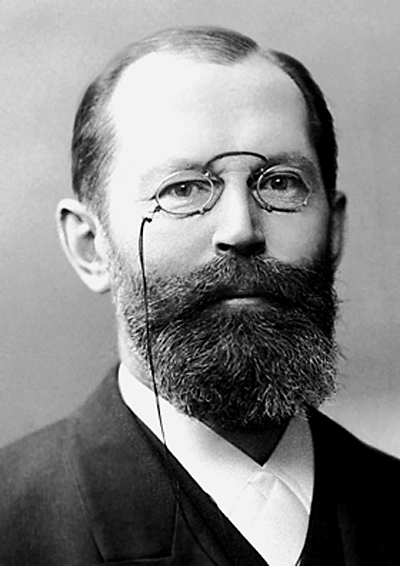
\includegraphics[width=\linewidth]{images/book3/fischer.jpg}
\end{minipage}\hfill
\begin{minipage}[t]{0.78\linewidth}
\vspace{0pt}
Emil Fischer, pada tahun 1891, telah menentukan konfigurasi glukosa dan
isomer-isomernya, sebelum ada metode fisika yang dapat melihat molekul:
dengan mengubah gula-gula satu menjadi yang lain dan menghitung
stereoisomer yang diperoleh. Proyeksi yang ia ciptakan untuk menuliskannya
masih menyandang namanya. Ia juga membuat \omterm{def:b2:biomolecules:peptide}{peptida} sintetis yang pertama, dan
menerima Hadiah Nobel Kimia 1902. (Potret: Atelier
Victoria, Berlin, sekitar 1895, domain publik; Wikimedia Commons.)
\end{minipage}
\end{history}

\section{Latihan}

\begin{exercise}[$\star$]\label{exo:b2:biomolecules:1}
Gambarlah alanina sebagai \omterm{def:b2:biomolecules:amino-acid}{zwitterion}, lalu bentuk-bentuk yang dominan pada pH 1 dan pada pH 12.
\end{exercise}

\begin{exercise}[$\star$]\label{exo:b2:biomolecules:2}
Hitunglah \omterm{def:b2:biomolecules:amino-acid}{titik isoelektrik} glisina, dan \omterm{def:b2:biomolecules:amino-acid}{titik isoelektrik} alanina ($\mathrm pK_a$ 2.35 dan 9.87).
\end{exercise}

\begin{exercise}[$\star$]\label{exo:b2:biomolecules:3}
Gambarlah dipeptida Ala--Gly dan lingkarilah \omterm{def:b2:biomolecules:peptide}{ikatan peptidanya}. Apa bedanya dengan Gly--Ala?
\end{exercise}

\begin{exercise}[$\star$]\label{exo:b2:biomolecules:4}
Dalam proyeksi Fischer dengan \ce{COOH} di atas dan \omterm{def:b2:biomolecules:amino-acid}{rantai samping} \ce{CH2OH}
di bawah,
\ce{NH2} serina mengarah ke kiri. Apakah serina itu D atau L? Tuliskan deskriptor CIP-nya.
\end{exercise}

\begin{exercise}[$\star\star$]\label{exo:b2:biomolecules:5}
Tentukan muatan bersih tripeptida Lys--Gly--Asp pada pH 1, 7, dan 12.
\end{exercise}

\begin{exercise}[$\star\star$]\label{exo:b2:biomolecules:6}
Mengapa \omterm{def:b2:biomolecules:peptide}{pereaksi kopling} dipakai untuk membentuk \omterm{def:b2:biomolecules:peptide}{ikatan peptida}, alih-alih
\omterm{def:b2:acyl-substitution:derivative}{asil klorida} asam amino terlindungi yang dibuat dengan tionil klorida dan
dipanaskan?
\end{exercise}

\begin{exercise}[$\star\star$]\label{exo:b2:biomolecules:7}
D-Fruktosa mengalami siklisasi melalui \ce{OH} C5-nya ke keton C2. Tentukan
ukuran cincinnya dan gambarlah
$\beta$-D-fruktofuranosa dalam \omterm{def:b2:biomolecules:anomer}{proyeksi Haworth}.
\end{exercise}

\begin{exercise}[$\star\star$]\label{exo:b2:biomolecules:8}
\omterm{def:b2:biomolecules:anomer}{Anomer-anomer} murni D-galaktosa mempunyai rotasi spesifik $+150.7$ ($\alpha$) dan $+52.8$ ($\beta$), dan
campuran kesetimbangannya $+80.2$ (data latihan). Hitunglah komposisi kesetimbangannya.
\end{exercise}

\begin{exercise}[$\star\star$]\label{exo:b2:biomolecules:9}
Jelaskan mengapa maltosa mereduksi larutan Fehling sedangkan sukrosa tidak,
dan mengapa sukrosa mereduksinya setelah dipanaskan dengan asam encer.
\end{exercise}

\begin{exercise}[$\star\star\star$]\label{exo:b2:biomolecules:10}
Bilangan penyabunan sebuah lemak adalah massa kalium hidroksida, dalam mg,
yang menyabunkan 1~g lemak itu. Hitunglah bilangan itu untuk triolein,
\ce{C57H104O6}, dan jelaskan mengapa lemak dengan rantai yang lebih pendek
mempunyai nilai yang lebih tinggi.
\end{exercise}

\begin{exercise}[$\star\star\star$]\label{exo:b2:biomolecules:11}
Rencanakan sintesis Gly--Ala dari glisina dan alanina: gugus pelindung,
aktivasi, kopling, pelepasan perlindungan, dengan sepasang gugus ortogonal.
\end{exercise}

\begin{exercise}[$\star\star\star$]\label{exo:b2:biomolecules:12}
Tuliskan untai yang komplementer dengan 5$'$-ATGCGT-3$'$, dari ujung 5$'$-nya,
dan hitunglah ikatan-ikatan hidrogen yang menahan untai ganda itu.
\end{exercise}

\section{Soal: Aspartam}

\begin{problem}[{Soal akhir pekan --- kedua asam amino dan konfigurasinya,
muatan dipeptida terhadap pH, sintesisnya dan masalah $\alpha$/$\beta$, serta
hidrolisisnya dalam minuman ringan}]
\label{pb:b2:biomolecules:1}
Aspartam adalah metil ester dipeptida yang dibentuk oleh gugus
$\alpha$-karboksilat asam L-aspartat
dengan gugus amino L-fenilalanina. Data: $\mathrm pK_a$ asam aspartat 2.0,
3.9, dan 9.9 (nilai model untuk gugus-gugus dipeptida). Massa molar
(\unit{g/mol}): C 12.011, H 1.008, N 14.007,
O 15.999.
% ledger: use:aspartame, pka:asp1, pka:asp2, pka:asp3, aw:C, aw:H, aw:N, aw:O

\medskip
\noindent\textbf{Bagian I --- Kedua asam amino.}
\begin{enumerate}
  \item Sebutkan ketiga senyawa yang dilepaskan oleh hidrolisis sempurna aspartam.
  \item Gambarlah asam L-aspartat dan L-fenilalanina dalam proyeksi Fischer.
  \item Tuliskan deskriptor CIP setiap pusat stereogenik.
  \item Berapa stereoisomer yang dimiliki aspartam?
  \item Gambarlah aspartam dan tandailah \omterm{def:b2:biomolecules:peptide}{ikatan peptida} dan esternya.
  \item Mengapa konfigurasi setiap asam amino penting bagi rasa manisnya?
\end{enumerate}

\medskip
\noindent\textbf{Bagian II --- Muatan terhadap pH.}
\begin{enumerate}[resume]
  \item Daftarlah gugus-gugus aspartam yang terionkan. Mengapa ujung-C tidak
        termasuk di antaranya?
  \item Dengan nilai-nilai model, tentukan muatan bersih pada pH 2.
  \item Hal yang sama pada pH 7.
  \item Hal yang sama pada pH 12.
  \item Perkirakan \omterm{def:b2:biomolecules:amino-acid}{titik isoelektrik} dalam model ini.
  \item Mengapa nilai $\mathrm pK_a$ dipeptida yang sesungguhnya akan
        berbeda dari nilai asam aspartat bebas?
\end{enumerate}

\medskip
\noindent\textbf{Bagian III --- Sintesis.}
\begin{enumerate}[resume]
  \item Mengapa asam aspartat dan metil ester fenilalanina tidak dapat begitu saja dipanaskan bersama?
  \item Gugus-gugus asam aspartat manakah yang harus dilindungi?
  \item Apa yang dilakukan \omterm{def:b2:biomolecules:peptide}{pereaksi kopling} pada gugus karboksilat yang bebas?
  \item Asam aspartat mempunyai dua gugus karboksilat. Apa yang terbentuk
        jika gugus yang salah yang dikopling?
  \item Usulkan perlindungan ortogonal yang hanya membiarkan gugus
        $\alpha$-karboksilat bebas, beserta pelepasannya.
  \item Mengapa asam amino yang teraktivasi tidak boleh dibiarkan terlalu
        lama dalam kondisi basa?
  \item Tuliskan urutan tahap-tahapnya.
\end{enumerate}

\medskip
\noindent\textbf{Bagian IV --- Hidrolisis dalam minuman ringan.}
\begin{enumerate}[resume]
  \item Ikatan-ikatan aspartam manakah yang dapat terhidrolisis dalam minuman
        yang asam? Manakah yang lebih dahulu?
  \item Tuliskan produk-produk hidrolisis esternya saja.
  \item Mengapa minuman yang sudah lama terasa kurang manis?
  \item Hitunglah massa molar aspartam, \ce{C14H18N2O5}.
  \item Hitunglah jumlah aspartam dalam sebuah kaleng yang mengandung \qty{180}{mg}.
  \item Nyatakan massa metanol yang dilepaskan oleh hidrolisis sempurna
        \qty{180}{mg} aspartam.
\end{enumerate}
\end{problem}
